\documentclass{article}
\usepackage[utf8]{inputenc}
\usepackage{graphicx}

\title{PS5}
\author{Amir Tayebi}
\date{\today}

\begin{document}

\maketitle

\section{Cleaning the data and plotting the associated party and gender against voting behavior}

Once again, I'm using the same website that I used for the previous homework assignment, but the data I scrapped this time is different. Here is my step by step explanations:
\begin{enumerate}
\item  getting the list of all candidates for all the states
\item getting bills from US Congress in year 2012 for all the states
\item looking for the term  "Education" in the title column
\item getting details of the bill
\item getting the actionId related to the passage of the bill
\item removing absentees
\item getting all the biographical data on all legislators associated with the bills
\item merging the biographical data with the votes
\item introducing some binary variable's additional variables for statistical analysis
\item plotting the relationship between the gender of a legislator and their voting behavior
\item plotting the relationship between the associated party of a legislator and their voting behavior

\end{enumerate}
The first graph shows the relationship between the gender of a legislator and their voting behavior in bills related to education. The width of the boxes represents the relative share of the each gender, while the height of the boxes shows the proportion of votes in each category(Yea or Nay).
The second graph shows the relationship between the associated party of a legislator and their voting behavior in bills related to education. Once again,the width of the boxes represents the relative share of the Democratic party relative to other parties, while the height of the boxes shows the proportion of votes in each category(Yea or Nay).
Since the two variables are binary variables, the mosaic plot is really usefull in understanding the relationship between the two variables.
\section{Mapping the share of female legislator}

This graph shows the share of female politicians by state. The mapped descriptive statistics show that in most states males are dominated in terms of county legislative offices.   




 

 
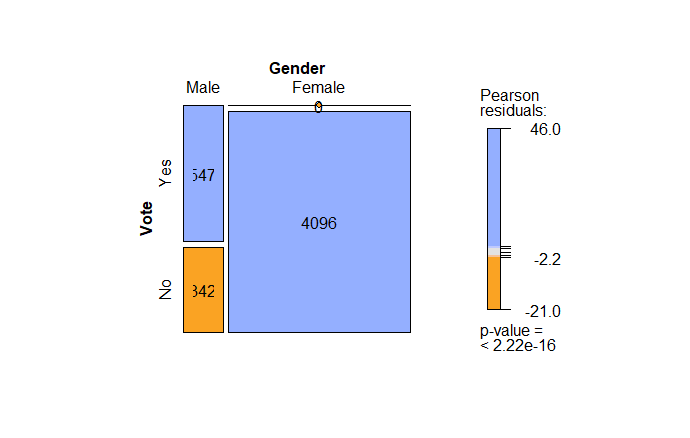
\includegraphics[width=\textwidth]{PS6a_Tayebi.png}
\begin{center}

Gender and Voting behavior
\end{center}


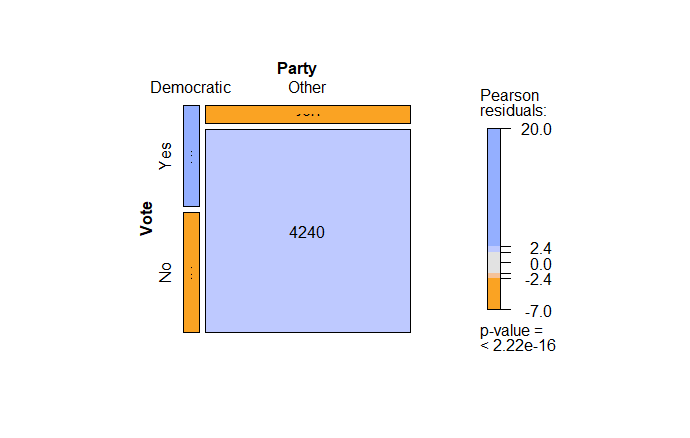
\includegraphics[width=\textwidth]{PS6b_Tayebi.png}
\begin{center}

Party and voting behavior
\end{center}

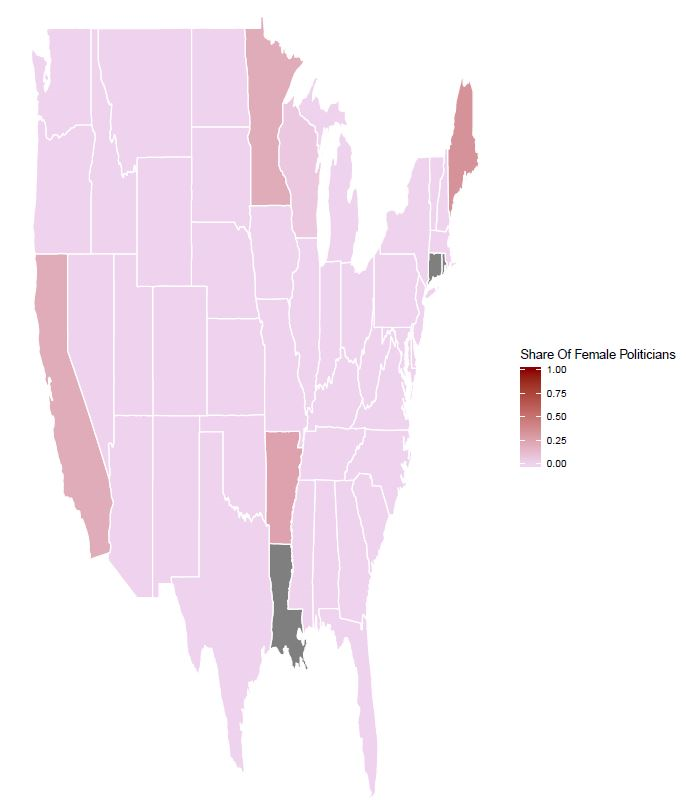
\includegraphics[width=\textwidth]{PS6c_Tayebi.png}
\begin{center}

Female Share in Politics
\end{center}
\end{document}

